
\documentclass[compress]{beamer}
\mode<presentation>
\usetheme{Warsaw}
\usecolortheme{seagull}
%\useoutertheme[subsection=false]{smoothbars}

\usepackage{stackengine}
%\setbeamertemplate{caption}{\raggedright\insertcaption\par}
\setbeamertemplate{caption}{\insertcaption} 
%\usepackage{caption}



%% ====================================== graphics
\newcommand{\smiley}{\tikz[baseline=-0.75ex,black]{
    \draw circle (2mm);
\node[fill,circle,inner sep=0.5pt] (left eye) at (135:0.8mm) {};
\node[fill,circle,inner sep=0.5pt] (right eye) at (45:0.8mm) {};
\draw (-145:0.9mm) arc (-120:-60:1.5mm);
    }
}

\newcommand{\frownie}{\tikz[baseline=-0.75ex,black]{
    \draw circle (2mm);
\node[fill,circle,inner sep=0.5pt] (left eye) at (135:0.8mm) {};
\node[fill,circle,inner sep=0.5pt] (right eye) at (45:0.8mm) {};
\draw (-145:0.9mm) arc (120:60:1.5mm);
    }
}

\newcommand{\neutralie}{\tikz[baseline=-0.75ex,black]{
    \draw circle (2mm);
\node[fill,circle,inner sep=0.5pt] (left eye) at (135:0.8mm) {};
\node[fill,circle,inner sep=0.5pt] (right eye) at (45:0.8mm) {};
\draw (-135:0.9mm) -- (-45:0.9mm);
    }
}


\usepackage{pgfplots}
\pgfplotsset{width=10cm,compat=1.9}
%\usepgfplotslibrary{external}
%\tikzexternalize
 \usepackage{pgfplotstable}

%\definecolor{markercolor}{RGB}{.49, 1, .63}
\definecolor{markercolor}{RGB}{124.9, 255, 160.65}

\pgfplotsset{
tick label style={font=\scriptsize},
label style={font=\scriptsize},
legend style={font=\scriptsize},
title style={font=\footnotesize}
}

%% ===========================================

\usetikzlibrary{calc}

%%% START MACRO FOR ANNOTATION OF TRIANGLE WITH SLOPE %%%.
\newcommand{\logLogSlopeTriangle}[5]
{
    % #1. Relative offset in x direction.
    % #2. Width in x direction, so xA-xB.
    % #3. Relative offset in y direction.
    % #4. Slope d(y)/d(log10(x)).
    % #5. Plot options.

    \pgfplotsextra
    {
        \pgfkeysgetvalue{/pgfplots/xmin}{\xmin}
        \pgfkeysgetvalue{/pgfplots/xmax}{\xmax}
        \pgfkeysgetvalue{/pgfplots/ymin}{\ymin}
        \pgfkeysgetvalue{/pgfplots/ymax}{\ymax}

        % Calculate auxilliary quantities, in relative sense.
        \pgfmathsetmacro{\xArel}{#1}
        \pgfmathsetmacro{\yArel}{#3}
        \pgfmathsetmacro{\xBrel}{#1-#2}
        \pgfmathsetmacro{\yBrel}{\yArel}
        \pgfmathsetmacro{\xCrel}{\xArel}

        \pgfmathsetmacro{\lnxB}{\xmin*(1-(#1-#2))+\xmax*(#1-#2)} % in [xmin,xmax].
        \pgfmathsetmacro{\lnxA}{\xmin*(1-#1)+\xmax*#1} % in [xmin,xmax].
        \pgfmathsetmacro{\lnyA}{\ymin*(1-#3)+\ymax*#3} % in [ymin,ymax].
        \pgfmathsetmacro{\lnyC}{\lnyA+#4*(\lnxA-\lnxB)}
        \pgfmathsetmacro{\yCrel}{\lnyC-\ymin)/(\ymax-\ymin)} % THE IMPROVED EXPRESSION WITHOUT 'DIMENSION TOO LARGE' ERROR.

        % Define coordinates for \draw. MIND THE 'rel axis cs' as opposed to the 'axis cs'.
        \coordinate (A) at (rel axis cs:\xArel,\yArel);
        \coordinate (B) at (rel axis cs:\xBrel,\yBrel);
        \coordinate (C) at (rel axis cs:\xCrel,\yCrel);

        % Draw slope triangle.
        \draw[#5]   (A)-- %node[pos=0.5,anchor=north] {1}
                    (B)-- 
                    (C)-- node[pos=0.5,anchor=west] {#4}
                    cycle;
    }
}
%%% END MACRO FOR ANNOTATION OF TRIANGLE WITH SLOPE %%%.

%%% START MACRO FOR ANNOTATION OF TRIANGLE WITH SLOPE %%%.
\newcommand{\logLogSlopeTriangleFlip}[5]
{
    % #1. Relative offset in x direction.
    % #2. Width in x direction, so xA-xB.
    % #3. Relative offset in y direction.
    % #4. Slope d(y)/d(log10(x)).
    % #5. Plot options.

    \pgfplotsextra
    {
        \pgfkeysgetvalue{/pgfplots/xmin}{\xmin}
        \pgfkeysgetvalue{/pgfplots/xmax}{\xmax}
        \pgfkeysgetvalue{/pgfplots/ymin}{\ymin}
        \pgfkeysgetvalue{/pgfplots/ymax}{\ymax}

        % Calculate auxilliary quantities, in relative sense.
        %\pgfmathsetmacro{\xArel}{#1}
        %\pgfmathsetmacro{\yArel}{#3}
        \pgfmathsetmacro{\xBrel}{#1-#2}
        \pgfmathsetmacro{\yBrel}{#3}
        \pgfmathsetmacro{\xCrel}{#1}

        \pgfmathsetmacro{\lnxB}{\xmin*(1-(#1-#2))+\xmax*(#1-#2)} % in [xmin,xmax].
        \pgfmathsetmacro{\lnxA}{\xmin*(1-#1)+\xmax*#1} % in [xmin,xmax].
        \pgfmathsetmacro{\lnyA}{\ymin*(1-#3)+\ymax*#3} % in [ymin,ymax].
        \pgfmathsetmacro{\lnyC}{\lnyA+#4*(\lnxA-\lnxB)}
        \pgfmathsetmacro{\yCrel}{\lnyC-\ymin)/(\ymax-\ymin)} % THE IMPROVED EXPRESSION WITHOUT 'DIMENSION TOO LARGE' ERROR.

        \pgfmathsetmacro{\xArel}{\xBrel}
        \pgfmathsetmacro{\yArel}{\yCrel}

        % Define coordinates for \draw. MIND THE 'rel axis cs' as opposed to the 'axis cs'.
        \coordinate (A) at (rel axis cs:\xArel,\yArel);
        \coordinate (B) at (rel axis cs:\xBrel,\yBrel);
        \coordinate (C) at (rel axis cs:\xCrel,\yCrel);

        % Draw slope triangle.
        \draw[#5]   (A)-- node[pos=0.5,anchor=east] {#4}
                    (B)-- 
                    (C)-- %node[pos=0.5,anchor=south] {1}
                    cycle;
    }
}
%%% END MACRO FOR ANNOTATION OF TRIANGLE WITH SLOPE %%%.


\useoutertheme{infolines}
\useinnertheme{rectangles}
\usepackage{hhline}
\setbeamercovered{dynamic}

\usepackage{soul}

\usepackage{array}
\usepackage{amsmath,amssymb,amsfonts,mathrsfs,amsthm}
\usepackage[utf8]{inputenc}
\usepackage{listings}
\usepackage{mathtools}
\usepackage{dsfont}
\usepackage{pdfpages}
%\usepackage[textsize=footnotesize,color=green]{todonotes}
\usepackage{algorithm, algorithmic}
\usepackage{bm}
\usepackage{tikz}
\usepackage[normalem]{ulem}

\usepackage{graphicx}
%\usepackage{subfigure}
\usepackage{subfig}
%\usepackage{caption}
%\usepackage{subcaption}

\usepackage{color}
\usepackage{pdflscape}
\usepackage{pifont}

\usepackage{bibentry}
\nobibliography*

%\usepackage[osf]{mathpazo}
%\usepackage{mathpazo}
%\renewcommand\rmdefault{ptm}
\newcommand*\diff[1]{\mathop{}\!{\mathrm{d}#1}}
\renewcommand{\topfraction}{0.85}
\renewcommand{\textfraction}{0.1}
\renewcommand{\floatpagefraction}{0.75}

\newcommand{\vect}[1]{\ensuremath\boldsymbol{#1}}
\newcommand{\tensor}[1]{\underline{\vect{#1}}}
\newcommand{\del}{\triangle}
\newcommand{\grad}{\nabla}
\newcommand{\curl}{\grad \times}
\renewcommand{\div}{\grad \cdot}
\newcommand{\ip}[1]{\left\langle #1 \right\rangle}
\newcommand{\eip}[1]{a\left( #1 \right)}
\newcommand{\td}[2]{\frac{{\rm d}#1}{{\rm d}#2}}
\newcommand{\pd}[3]{\frac{\partial^{#3} #1}{\partial#2^{#3}}}
\newcommand{\pdd}[2]{\frac{\partial^2#1}{\partial#2^2}}

\newcommand{\circone}{\ding{192}}
\newcommand{\circtwo}{\ding{193}}
\newcommand{\circthree}{\ding{194}}
\newcommand{\circfour}{\ding{195}}
\newcommand{\circfive}{\ding{196}}

\newcommand{\Reyn}{\rm Re}

\newcommand{\bs}[1]{\boldsymbol{#1}}
\DeclareMathOperator{\diag}{diag}

\newcommand{\equaldef}{\stackrel{\mathrm{def}}{=}}


\newcommand{\mb}[1]{\mathbf{#1}}
\newcommand{\mbb}[1]{\mathbb{#1}}
\newcommand{\mc}[1]{\mathcal{#1}}
\newcommand{\nor}[1]{\left\| #1 \right\|}
\newcommand{\snor}[1]{\left| #1 \right|}
\newcommand{\Grad} {\ensuremath{\nabla}}
\newcommand{\Div} {\ensuremath{\nabla\cdot}}
\newcommand{\Nel} {\ensuremath{{N^\text{el}}}}
\newcommand{\jump}[1] {\ensuremath{\LRs{\![#1]\!}}}
\newcommand{\avg}[1] {\ensuremath{\LRc{\!\{#1\}\!}}}

\newcommand{\uh}{\widehat{u}}
\newcommand{\fnh}{\widehat{f}_n}
\renewcommand{\L}{L^2\LRp{\Omega}}
\newcommand{\pO}{\partial\Omega}
\newcommand{\Gh}{\Gamma_h}
\newcommand{\Gm}{\Gamma_{-}}
\newcommand{\Gp}{\Gamma_{+}}
\newcommand{\Go}{\Gamma_0}
\newcommand{\Oh}{\Omega_h}

%\newcommand{\nor}[1]{\left\| #1 \right\|}
%\newcommand{\snor}[1]{\left| #1 \right|}
\newcommand{\LRp}[1]{\left( #1 \right)}
\newcommand{\LRs}[1]{\left[ #1 \right]}
\newcommand{\LRa}[1]{\left\langle #1 \right\rangle}
\newcommand{\LRb}[1]{\left| #1 \right|}
\newcommand{\LRc}[1]{\left\{ #1 \right\}}



\newcommand{\bibfoot}[1]{\footnote{\tiny\bibentry{#1}}}
\renewcommand{\note}[1]{\textcolor{red}{{#1}}}

\newcommand{\eval}[2][\right]{\relax
  \ifx#1\right\relax \left.\fi#2#1\rvert}

\def\etal{{\it et al.~}}


\def\arr#1#2#3#4{\left[
\begin{array}{cc}
#1 & #2\\
#3 & #4\\
\end{array}
\right]}
\def\vecttwo#1#2{\left[
\begin{array}{c}
#1\\
#2\\
\end{array}
\right]}
\def\vectthree#1#2#3{\left[
\begin{array}{c}
#1\\
#2\\
#3\\
\end{array}
\right]}
\def\vectfour#1#2#3#4{\left[
\begin{array}{c}
#1\\
#2\\
#3\\
#4\\
\end{array}
\right]}

\newcommand{\G} {\Gamma}
\newcommand{\Gin} {\Gamma_{in}}
\newcommand{\Gout} {\Gamma_{out}}

%\newcommand\blfootnote[1]{%
%  \begingroup
%  \renewcommand\thefootnote{}\footnote{#1}%
%  \addtocounter{footnote}{-1}%
%  \endgroup
%}

% removes nav symbols
\beamertemplatenavigationsymbolsempty
%\setbeamertemplate{caption}{\raggedright\insertcaption\par}

% defines newblock as null, giving compile issues otherwise
\let\newblock\relax 


%\title[WADG]{Weight-adjusted discontinuous Galerkin methods for heterogeneous media and curvilinear meshes}
\title[WADG]{Weight-adjusted discontinuous Galerkin methods for acoustic and elastic wave propagation}
\date[February 28, 2017]{Rice Oil and Gas HPC Conference 2017\\March 15, 2017}
\author[Chan, Hewett, Warburton]{Jesse Chan\inst{1}, Russell Hewett\inst{2}, T.\ Warburton\inst{3}}
\institute[CAAM]{\inst{1}Department of Computational and Applied Math, Rice University\\ \inst{2}TOTAL E\&P Research and Technology USA\\ \inst{3}Department of Mathematics, Virginia Tech}

\pgfplotstableread[col sep=space]{
N V S T
1   9.3794e-01   8.1757e-01   8.9829e-01
2   1.1345e+00   1.4601e+00   1.2199e+00
3   1.4877e+00   1.5730e+00   1.3218e+00
4   2.5118e+00   1.8765e+00   1.6277e+00
5   3.4739e+00   2.1611e+00   1.9112e+00
6   5.1833e+00   2.5859e+00   2.3807e+00
7   7.4018e+00   2.3500e+00   2.5861e+00
8   1.0194e+01   2.6710e+00   3.1296e+00
9   1.6618e+01   2.7522e+00   3.9489e+00
      }\runtimeNaive

\pgfplotstableread[col sep=space]{
N V S T
    1    0.9379    0.3507    0.5409
    2    1.1345    0.7825    0.8923
    3    1.4877    1.0923    1.1204
    4    2.5118    1.5340    1.4873
    5    3.4739    1.8295    1.7745
    6    5.1833    3.3931    2.6688
    7    7.4018    2.9729    2.9017
    8   10.1935    3.6607    3.6572
    9   16.6176    5.8237    5.6122

}\runtimeOptNaive
   
% runtime
\pgfplotstableread[col sep=space]{
N V S T
1    0.8865    1.8615    0.8886
2    0.8992    2.4076    1.1769
3    1.0099    2.5900    1.2355
4    1.6471    2.3605    1.4801
5    1.7538    2.2007    1.6203
6    2.8192    2.2626    2.0068
7    4.0938    1.8900    2.1282
8    6.3871    1.7606    2.6168
9    7.6471    2.3645    2.8213
}\runtimeBlocked

\pgfplotstableread[col sep=space]{
N V S F
%1    0.3067    0.2467    0.0584
%2    0.6890    0.5917    0.0461
%3    1.2947    1.1235    0.0432
%4    1.3824    1.7513    0.0402
%5    1.8976    1.7048    0.0379
%6    1.9774    1.7700    0.0374
%7    1.9683    1.9610    0.0354
%8    1.7695    2.0670    0.0346
%9    1.9443    2.0914    0.0335
1    0.3067    0.2019    0.0584
 2   0.6890    0.4637    0.0461
3    1.2947    0.8537    0.0432
4    1.3824    1.2417    0.0402
5    1.8976    1.4066    0.0379
6    1.9774    1.4887    0.0374
7    1.9683    1.5675    0.0354
8    1.7695    1.8836    0.0346
9    1.9443    1.2083    0.0335
}\GFLOPSBlockNodal

\pgfplotstableread[col sep=space]{
N V S F
1 167.0430  172.5100  133.3820
 2 166.2430  172.1310  142.1890
3  164.0040  172.0910  138.8410
4  111.7100  160.8480  127.9770
5  131.0690  169.5880  123.7740
6  121.5190  131.0820  127.9820
7  124.2650  134.2170  118.5400
8  157.7240  157.9600  115.3520
9  122.9810  122.0410  115.9380
%1   1.6704e+02   1.7034e+02   1.3338e+02
% 2  1.6624e+02   1.7079e+02   1.4219e+02
%  3 1.6400e+02   1.6996e+02   1.3884e+02
% 4  1.1171e+02   1.6262e+02   1.2798e+02
% 5  1.3107e+02   1.6678e+02   1.2377e+02
% 6  1.2152e+02   1.2184e+02   1.2798e+02
% 7  1.2427e+02   1.3592e+02   1.1854e+02
% 8  1.5772e+02   1.5000e+02   1.1535e+02
% 9  1.2298e+02   1.1462e+02   1.1594e+02
}\BWBlockNodal

\pgfplotstableread[col sep=space]{
N V S
1  0.3048    0.2552
 2   0.5607    0.3123
  3  0.8919    0.5365
 4   0.9145    0.6203
 5   0.9433    0.6689
 6   1.0493    0.7259
 7   1.0487    0.7876
 8   1.0338    0.8112
 9   0.8529    0.8612
 }\GFLOPSNodal

\pgfplotstableread[col sep=space]{
N V Vopt S
1  1.6440e+02   1.6632e+02   1.3286e+02
2   1.5096e+02   1.6659e+02   9.4100e+01
3   1.0639e+02   1.6105e+02   8.0230e+01
4   6.8770e+01   9.6448e+01   6.6073e+01
 5  4.7656e+01   1.2547e+02   5.3975e+01
6   3.3726e+01   1.1956e+02   3.9934e+01
7   2.3302e+01   1.1047e+02   3.2720e+01
8   1.7389e+01   1.0452e+02   2.6895e+01
9   1.0300e+01   1.4811e+02   2.2290e+01
   }\BWNodal
   
\pgfplotstableread[col sep=space]{
N V S
1    0.4218    0.1847
2    0.4998    0.3181
3    0.5860    0.4434
4    0.6122    0.4898
5    0.5616    0.5256
6    0.6316    0.6190
7    0.6372    0.5710
8    0.6331    0.6379
9    0.6414    0.6747
}\GFLOPSBern

\pgfplotstableread[col sep=space]{
N V S
1  156.0280  108.2120
2  167.7100  132.0770
3  167.4290  133.0320
4  168.5340  118.4780
5  168.7020  118.7510
6  170.3240  104.9450
7  170.4290   76.6690
8  169.2200   70.1780
9  170.6090   61.6120
}\BWBern


\begin{document}


\begin{frame}
\maketitle
\end{frame}

\frame{
\frametitle{High order DG methods for wave propagation}
\setcounter{subfigure}{0}
\vspace{-1em}
\begin{columns}
\begin{column}{.5\textwidth}
\begin{itemize}
\item<1-> Unstructured (tetrahedral) meshes for geometric flexibility.
\vspace{.5em}
\item<2-> Low numerical dissipation and dispersion.
\vspace{.5em}
\item<4-> High order approximations: more accurate per unknown.
\vspace{.5em}
\item<5-> Explicit time stepping: high performance on many-core.
\end{itemize}
\end{column}
\begin{column}{.475\textwidth}
\begin{figure}
\centering
\begin{overlayarea}{\textwidth}{.5\textheight}
\only<1>{
\vspace{-2em}\includegraphics[width=.95\textwidth]{figs/wave.png}
\caption*{Figure courtesy of Axel Modave.}
}
\only<2>{
\includegraphics[width=.95\textwidth]{figs/wave_N1.eps}
\caption*{\textbf{Fine} linear approximation.}
}
\only<3>{
\includegraphics[width=.95\textwidth]{figs/wave_N2.eps}
\caption*{\textbf{Coarse} quadratic approximation.}
}
\only<4>{
\includegraphics[width=.95\textwidth]{figs/error_v_dofs.png}
\caption*{Max errors vs.\ dofs.}
}
\only<5>{
\includegraphics[width=.975\textwidth]{figs/gpu.pdf}
\caption*{Graphics processing units (GPU).}
}
%\caption*{Image courtesy of Axel Modave.}
\end{overlayarea}
\end{figure}
\end{column}
\end{columns}

}


%\frame{
%\frametitle{Efficient implementations of DG}
%
%\begin{itemize}
%\item Quadrature-free implementation on \textbf{simplicial} meshes: \only<1>{$c^2$}\only<2->{\note{$c^2$}}, \only<1>{$J, J^f$}\only<2->{\note{$J, J^f$}} piecewise constant (non-curved meshes).  
%\begin{overlayarea}{.875\textwidth}{.35\textheight}
%\only<1>{
%\begin{align*}
%\int_{D^k}\frac{1}{c^2}\pd{p}{t}{} q &= \int_{D^k} \Div \bm{u} q  + \frac{1}{2}\int_{\partial D^k} \LRp{\jump{\bm{u}}\cdot{\bm{n}} + \tau_p\jump{p}} q\\
%\int_{D^k}\pd{\bm{u}}{t}{} \bm{v} &= \int_{D^k} \Grad p \cdot \bm{v} + \frac{1}{2}\int_{\partial D^k} \LRp{\jump{p} + \tau_u\jump{\bm{u}}\cdot\bm{n}} \bm{v}
%\end{align*}
%}
%\only<2>{
%\begin{align*}
%\int_{\widehat{D}}\note{\frac{1}{c^2}}\pd{p}{t}{} q \note{J} &= \int_{\widehat{D}} \Div \bm{u} q\note{J}  + \frac{1}{2}\int_{\partial \widehat{D}} \LRp{\jump{\bm{u}}\cdot{\bm{n}} + \tau_p\jump{p}} q\note{J^f}\\
%\int_{\widehat{D}}\pd{\bm{u}}{t}{} \bm{v} \note{J} &= \int_{\widehat{D}} \Grad p \cdot \bm{v}\note{J} + \frac{1}{2}\int_{\partial \widehat{D}} \LRp{\jump{p} + \tau_u\jump{\bm{u}}\cdot\bm{n}} \bm{v}\note{J^f}
%\end{align*}
%}
%\only<3>{
%\begin{align*}
%\note{\frac{J}{c^2}}\int_{\widehat{D}}\pd{p}{t}{} q  &= \note{J}\int_{\widehat{D}} \Div \bm{u} q  + \note{J^f}\frac{1}{2}\int_{\partial \widehat{D}} \LRp{\jump{\bm{u}}\cdot{\bm{n}} + \tau_p\jump{p}} q\\
%\note{J}\int_{\widehat{D}}\pd{\bm{u}}{t}{} \bm{v}  &= \note{J}\int_{\widehat{D}} \Grad p \cdot \bm{v} + \note{J^f}\frac{1}{2}\int_{\partial \widehat{D}} \LRp{\jump{p} + \tau_u\jump{\bm{u}}\cdot\bm{n}} \bm{v}
%\end{align*}
%}
%\end{overlayarea}
%\item Variable $c^2, J$ on quads, hexes: GLL nodes + mass lumping.   
%\item Triangles and tets: require special nodal sets to maintain high order accuracy and stability.  
%\end{itemize}
%}

\frame{
\frametitle{High order approximation of media and geometry}
\setcounter{subfigure}{0}
\begin{itemize}
\item Efficient implementations on \textbf{triangular} or \textbf{tetrahedral} meshes: piecewise constant wavespeed $c^2$, non-curved meshes.  
%\vspace{.1em}
%\begin{align*}
%\only<1>{
%\int_{D^k}\frac{1}{c^2}\pd{p}{t}{} q &= \int_{D^k} \Div \bm{u} q  + \frac{1}{2}\int_{\partial D^k} \LRp{\jump{\bm{u}}\cdot{\bm{n}} + \tau_p\jump{p}} q\\
%\int_{D^k}\pd{\bm{u}}{t}{} \bm{v} &= \int_{D^k} \Grad p \cdot \bm{v} + \frac{1}{2}\int_{\partial D^k} \LRp{\jump{p} + \tau_u\jump{\bm{u}}\cdot\bm{n}} \bm{v}
%}
%\only<2>{
%\int_{\widehat{D}}\note{\frac{1}{c^2}}\pd{p}{t}{} q \note{J} &= \int_{\widehat{D}} \Div \bm{u} q\note{J}  + \frac{1}{2}\int_{\partial \widehat{D}} \LRp{\jump{\bm{u}}\cdot{\bm{n}} + \tau_p\jump{p}} q\note{J^f}\\
%\int_{\widehat{D}}\pd{\bm{u}}{t}{} \bm{v} \note{J} &= \int_{\widehat{D}} \Grad p \cdot \bm{v}\note{J} + \frac{1}{2}\int_{\partial \widehat{D}} \LRp{\jump{p} + \tau_u\jump{\bm{u}}\cdot\bm{n}} \bm{v}\note{J^f}
%}
%\only<3>{
%\note{\frac{J}{c^2}}\int_{\widehat{D}}\pd{p}{t}{} q  &= \note{J}\int_{\widehat{D}} \Div \bm{u} q  + \note{J^f}\frac{1}{2}\int_{\partial \widehat{D}} \LRp{\jump{\bm{u}}\cdot{\bm{n}} + \tau_p\jump{p}} q\\
%\note{J}\int_{\widehat{D}}\pd{\bm{u}}{t}{} \bm{v}  &= \note{J}\int_{\widehat{D}} \Grad p \cdot \bm{v} + \note{J^f}\frac{1}{2}\int_{\partial \widehat{D}} \LRp{\jump{p} + \tau_u\jump{\bm{u}}\cdot\bm{n}} \bm{v}
%}
%\end{align*}
\vspace{1em}
\item Spurious reflections for low order approximations of media, geometry.
\end{itemize}
\vspace{-.75em}
\begin{figure}
\subfloat[Mesh and exact $c^2$]{\includegraphics[width=.34\textwidth]{figs/c2WADG.png}}
%\hspace{.1em}
\subfloat[Piecewise const.\ $c^2$]{\includegraphics[width=.3\textwidth]{figs/p0WADG.png}}
\hspace{.25em}
\subfloat[High order $c^2$]{\includegraphics[width=.3\textwidth]{figs/pNWADG.png}}
\end{figure}

}


%\frame{
%\frametitle{High order approximation of media and geometry}
%\begin{itemize}
%\item $c^2(\bm{x})$ often assumed piecewise constant for efficiency.
%\vspace{.5em}
%\item Discontinuities in $c^2(\bm{x})$ can result in spurious reflections.
%\vspace{.5em}
%\item Analogous problems with planar approximation of curved geometry.
%\end{itemize}
%
%\begin{figure}
%\subfloat[Mesh and exact $c^2$]{\includegraphics[width=.31\textwidth]{figs/c2WADG.png}}
%\hspace{.2em}
%\subfloat[Piecewise constant $c^2$]{\includegraphics[width=.31\textwidth]{figs/p0WADG.png}}
%\hspace{.2em}
%\subfloat[High order $c^2$]{\includegraphics[width=.31\textwidth]{figs/pNWADG.png}}
%\end{figure}
%
%}

\section{Weight-adjusted DG methods}

\begin{frame}[noframenumbering]
  \frametitle{Outline}
\only<1>{
 \tableofcontents
}
\only<2>{
 \tableofcontents[currentsection]
}
\end{frame}

\frame{
\frametitle{Energy stable discontinuous Galerkin formulations}

\begin{itemize}
\item Model problem: acoustic wave equation (pressure-velocity system)
\begin{align*}
\frac{1}{c^2(\bm{x})}\pd{p}{t}{} = \Div \bm{u}, \qquad \pd{\bm{u}}{t}{} = \Grad p
\end{align*}
\item Local formulation 
\begin{align*}
\int_{D^k}\frac{1}{c^2(\bm{x})}\pd{p}{t}{} q &= \int_{D^k} \Div \bm{u} q  + \frac{1}{2}\int_{\partial D^k} \LRp{\jump{\bm{u}}\cdot{\bm{n}} + \tau_p\jump{p}} q\\
\int_{D^k}\pd{\bm{u}}{t}{} \bm{v} &= \int_{D^k} \Grad p \cdot \bm{v} + \frac{1}{2}\int_{\partial D^k} \LRp{\jump{p} + \tau_u\jump{\bm{u}}\cdot\bm{n}} \bm{v}
\end{align*}
\item High order accuracy, semi-discrete energy stability
\[
\pd{}{t}{}\LRp{\sum_{k} \int_{D^k} \frac{p^2}{c^2(\bm{x})} + \LRb{\bm{u}}^2} = -\sum_k\int_{\partial D^k} \tau_p\jump{p}^2 +  \tau_u\jump{\bm{u}\cdot\bm{n}}^2 \leq 0.
\]
\end{itemize}
}


\frame{
\frametitle{Weighted mass matrices}
\begin{itemize}
\item Spatially varying weights appear in DG mass matrices
\[
\only<1,5>{\int_{D^k}{\frac{1}{c^2}}\pd{p}{t}{} q = \text{pressure RHS}, \qquad \int_{D^k}\pd{\bm{u}}{t}{} \bm{v} = \text{velocity RHS}}
\only<2>{\int_{\note{\widehat{D}}}{\frac{1}{c^2}}\pd{p}{t}{} q {J} = \text{pressure RHS}, \qquad \int_{\note{\widehat{D}}}\pd{\bm{u}}{t}{} \bm{v} {J} = \text{velocity RHS}}
\only<3>{\int_{\widehat{D}}{\frac{1}{c^2}}\pd{p}{t}{} q \note{J} =  \text{pressure RHS}, \qquad \int_{\widehat{D}}\pd{\bm{u}}{t}{} \bm{v} \note{J} = \text{velocity RHS}}
\only<4>{\int_{\widehat{D}}\note{\frac{1}{c^2}}\pd{p}{t}{} q \note{J} =  \text{pressure RHS}, \qquad \int_{\widehat{D}}\pd{\bm{u}}{t}{} \bm{v} \note{J} = \text{velocity RHS}}
\]
\item \only<1-2,4->{Curvilinear}\only<3>{\textcolor{red}{Curvilinear}} meshes and wave propagation in \only<1-3,5>{heterogeneous media}\only<4>{\textcolor{red}{heterogeneous media}} 
\begin{overlayarea}{\textwidth}{.25\textheight}
\vspace{-1.25em}
\only<1-2,5>{
\begin{align*}
\LRp{\bm{M}_{w}}_{ij} &= \int_{\widehat{D}}\phi_i \phi_j w(x),\\
\td{}{t}\bm{M}_{w} \bm{u} &= \text{right hand side}.
\end{align*}
}
\only<3>{
\begin{align*}
\LRp{\bm{M}_{w}}_{ij} &= \int_{\widehat{D}}\phi_i \phi_j \textcolor{red}{J(x)}, \\
\td{}{t}\bm{M}_{\textcolor{red}{J}} \bm{u} &= \text{right hand side}.
\end{align*}
}
\only<4>{
\begin{align*}
\LRp{\bm{M}_{w}}_{ij} &= \int_{\widehat{D}}\phi_i \phi_j \textcolor{red}{\frac{J}{c^{2}(x)}}, \\
\td{}{t}\bm{M}_{\textcolor{red}{J/c^2}} \bm{u} &= \text{right hand side}.
\end{align*}
}
\end{overlayarea}
\item Inherits \textbf{high order accuracy} and \textbf{energy stability} with respect to a weighted $L^2$ norm, but requires $\bm{M}_w^{-1}$ explicitly \only<1-4>{over each element}\only<5>{\textcolor{red}{over each element}}.
\vspace{.5em}
\item On-the-fly assembly + inversion or pre-computation and \only<1-4>{storage}\only<5>{\note{storage}}.
\end{itemize}
}

%\frame{
%\frametitle{Inverting weighted mass matrices: storage costs}
%
%\begin{itemize}
%\item Assembling and inverting $\bm{M}_w$ on-the-fly
%\begin{itemize}
%\item High computational complexity w.r.t.\ $N$.
%\item Fine-grain parallelization of solve more difficult.
%\end{itemize}
%\vspace{1em}
%\item Pre-computation and storage of $\bm{M}_w^{-1}$ 
%\begin{itemize}
%\item Increase from $O(N^3)$ to $O(N^6)$ storage per element.
%\end{itemize}
%\end{itemize}
%\vspace{2em}
%Memory costs of DG (\emph{single precision}, one field, 3D tets, 1M elements):
%\begin{table}
%\centering                                                                                   
%\begin{tabular}{| c | c | c | c | c |}
%\hline
%Order $N$ & $N=1$ & $N=3$ & $N=5$ & $N=7$ \\
%\hline
%Block matrix $M^{-1}$ & .298 GB  & \textcolor{red}{3.2 GB}  & \textcolor{red}{25.08 GB} & \textcolor{red}{115.2 GB} \\
%\hline
%Solution dofs & .075 GB  & .16 GB  & .448 GB & .96 GB \\
%\hline 
%\end{tabular}
%\label{table:cost}
%\end{table}
%%\begin{center}
%%Large storage costs at high order: need mass matrix inverses if $w = w(\bm{x})$.  \textcolor{red}{Inefficient for accelerator architectures!}
%%\end{center}
%}

\frame{
\frametitle{Weight-adjusted DG: convergence and implementation}
\begin{itemize}
\item \textcolor{red}{Weight-adjusted DG (WADG)}: energy stable approximation of weighted mass matrix  
\[
\bm{M}_{w}\td{\bm{U}}{t} \approx \textcolor{red}{{\bm{M}} \LRp{{\bm{M}}_{1/w}}^{-1} {\bm{M}}} \td{\bm{U}}{t} = \text{right hand side}.
\]
\item WADG \textit{a-priori} estimates: optimal weighted projection estimate shows \textbf{high order accuracy}:
\begin{align*}
&\nor{u - P_w u}_{L^2} \leq C h^{N+1}  \nor{w}_{W^{N+1,\infty}} \nor{\frac{\sqrt{J}}{w}}_{L^{\infty}} \nor{u}_{W^{N+1,2}}.
\end{align*}
\item Bypasses inverse of weighted matrix $\LRp{\bm{M}_{w}}^{-1}$ 
\[
\LRp{{\bm{M}} \LRp{{\bm{M}}_{1/w}}^{-1}{\bm{M}}}^{-1} = {\bm{M}}^{-1} {{\bm{M}}}_{1/w} {\bm{M}}^{-1}.
\]
\end{itemize}
}

\frame{
\frametitle{A non-intrusive and low-storage implementation}
\begin{itemize}
\item Operator evaluation reuses implementation for $w=1$
\begin{align*}
{\bm{M}} \LRp{{\bm{M}}_{1/w}}^{-1} {\bm{M}} \td{\bm{U}}{t} &= \bm{A}_h \bm{U} \\
\rightarrow \LRp{{\bm{M}}_{1/w}}^{-1} {\bm{M}} \td{\bm{U}}{t} &= \underbrace{\bm{M}^{-1}\bm{A}_h \bm{U} }_{\text{RHS for }w = 1}
\end{align*}
%\vspace{.25em}
\item Low storage: matrix-free application of $\bm{M}^{-1}{\bm{M}}_{1/w}$.  
\[
\LRp{\bm{M}}^{-1} {\bm{M}}_{1/w}\text{RHS} = \underbrace{\widehat{\bm{M}}^{-1} \bm{V}_q^T W}_{\bm{P}_q} {\rm diag}\LRp{1/w} \bm{V}_q \LRp{\text{RHS}}.
\]
\item Non-intrusive: modify RHS locally before update.  For non-curved meshes, can combine with \textit{optimal complexity} RHS evaluation.\footnotemark
\end{itemize}

\let\thefootnote\relax\footnotetext{\tiny Chan, Warburton 2015.  {GPU-accelerated Bernstein-Bezier discontinuous Galerkin methods for wave propagation}.}
}


%\frame{
%\frametitle{Weight-adjusted DG: not locally conservative}
%
%\begin{itemize}
%\item \textcolor{red}{Con:} loss of local conservation for $w(x) \not\in P^N$!
%\vspace{1em}
%\item \textcolor{blue}{Pro:} superconvergence of conservation error
%\begin{align*}
%\text{Conservation error}
%&\leq C \textcolor{red}{h^{2N+2}} \nor{w}_{W^{N+1,\infty}}\nor{p}_{W^{N+1,2}}
%\end{align*}
%where $C$ depends on mesh quality and max/min values of $w$.
%\vspace{1em}
%\item \textcolor{blue}{Pro:} can restore local conservation with rank-1 update (Shermann-Morrison).
%\end{itemize}
%}

\section{Acoustic wave propagation}

\begin{frame}[noframenumbering]
    \frametitle{Outline}
    \tableofcontents[currentsection]
\end{frame}


\frame{
\frametitle{Acoustic wave equation: variable coefficients}
\setcounter{subfigure}{0}
%\vspace{.5em}

\begin{figure}
\centering
\only<1>{
\subfloat[$c^2(x,y)$]{
\includegraphics[width=.325\textwidth]{figs/cfun.png}
}
\hspace{1em}
\subfloat[Standard DG]{
\includegraphics[width=.325\textwidth]{figs/cmass_wave.png}
}}
\only<2>{
\subfloat[$c^2(x,y)$]{
\includegraphics[width=.325\textwidth]{figs/cfun.png}
}
\hspace{1em}
\subfloat[Weighted-adjusted DG]{
\includegraphics[width=.325\textwidth]{figs/cproj_wave.png}
}}
\caption{Standard vs.\ weight-adjusted DG with spatially varying $c^2$ containing both smooth variations and a discontinuity.}
\end{figure}
}



\frame{
\frametitle{Acoustics, variable coefficients: $L^2$ errors}
\setcounter{subfigure}{0}
\vspace{.5em}
Smooth wavefield $c^2(x,y) = 1 + \frac{1}{2}\sin(\pi x)\sin(\pi y)$
\only<1>{
\begin{table}
\centering                                                                                   
\begin{tabular}{c||c|c|c|c|}
\hline                                                   
 & $h = 1$ & $h = 1/2$ & $h = 1/4$ & $h = 1/8$\\ 
\hline                                                   
DG $N = 1$ &   2.13e-01 & 6.25e-02 & 1.64e-02 & 4.19e-03 \\
\hline
WADG $N = 1$ &  2.05e-01 & 5.99e-02 & 1.62e-02 & 4.18e-03 \\
%\hhline{=====}                              
\hline \\ \hline
DG $N = 2$ &  3.01e-02 & 3.60e-03 & 4.21e-04 & 5.07e-05 \\
\hline                                                   
WADG $N = 2$ &  2.89e-02 & 3.54e-03 & 4.18e-04 & 5.07e-05 \\
%\hhline{|=||=|=|=|=|}                                   
\hline \\ \hline
DG $N = 3$ &   6.10e-03 & 3.33e-04 & 2.04e-05 & 1.22e-06 \\
\hline                                                   
WADG $N = 3$ &   8.69e-03 & 3.47e-04 & 2.03e-05 & 1.22e-06 \\
%\hhline{|=||=|=|=|=|}                            
\hline \\ \hline
DG $N = 4$ &  6.61e-04 & 2.12e-05 & 6.39e-07 & 1.94e-08 \\
\hline                                                   
WADG $N = 4$ & 1.09e-03 & 2.27e-05 & 6.30e-07 & 1.93e-08 \\
\hline                                                   
\end{tabular}

\caption{Convergence of standard, weight-adjusted DG to a manufactured solution.}
\label{table:manusol}
\end{table}
}
\only<2>{
\begin{table}
\centering
%\subfloat[Standard DG, reference solution (spectral method)]{
\begin{tabular}{c||c|c|c|c|}
\hline                                                   
 & $h = 1$ & $h = 1/2$ & $h = 1/4$ & $h = 1/8$\\ 
\hline                                                   
DG $N = 1$ &   2.48e-01 & 7.58-02 & 1.69e-02 & 4.46e-03 \\
\hline                                                
WADG $N = 1$ &  2.50e-01 & 7.72e-02 & 1.69e-02 & 4.47e-03 \\
%\hhline{|=||=|=|=|=|}
\hline \\ \hline
DG $N = 2$ &  5.95e-02 & 9.95e-03 & 1.10e-03 & 1.22e-04 \\
\hline                                                   
WADG $N = 2$ &  6.09e-02 & 1.02e-02 & 1.10e-03 & 1.22e-04 \\
%\hhline{|=||=|=|=|=|}
\hline \\ \hline
DG $N = 3$ &   2.29e-02 & 1.98e-03 & 9.52e-05 & 6.56e-06 \\
\hline                                                   
WADG $N = 3$ &   1.98e-02 & 1.98e-03 & 9.52e-05 & 6.56e-06 \\
%\hhline{|=||=|=|=|=|}                              
\hline \\ \hline
DG $N = 4$ &  4.90e-03 & 3.01e-04 & 1.78e-05 & 7.27e-07 \\
\hline                                                   
WADG $N = 4$ & 4.64e-03 & 3.02e-04 & 1.78e-05 & 7.28e-07 \\
\hline 
\end{tabular}
%}\\
%\subfloat[Weighted DG, reference solution (spectral method)]{
%\begin{tabular}{|c||c|c|c|c|}
%\hline                                                   
% & $h = 1$ & $h = 1/2$ & $h = 1/4$ & $h = 1/8$\\ 
%\hline 
%\end{tabular}
%}
\caption{Convergence to a reference solution ($N = 100$ spectral method).}
\label{table:rates}
\end{table}
}
}

\frame{
\frametitle{Acoustics, variable coefficients: convergence}
\setcounter{subfigure}{0}

\begin{table}
\centering
\subfloat[Rates of convergence to manufactured solution]{
\begin{tabular}{|c||c|c|c|c|}
\hline                                                   
 & $N = 1$ & $N = 2$ & $N = 3$ & $N = 4$\\ 
\hline                                                   
DG&       1.9220  &     3.0752     &      4.0440      &      5.0446    \\
\hline                                                   
WADG &  1.9211 &     3.0629     &    4.0752    &   5.0990\\
\hline 
\end{tabular}
}\\
\subfloat[Rates of convergence to reference solution]{
\begin{tabular}{|c||c|c|c|c|}
\hline                                                   
 & $N = 1$ & $N = 2$ & $N = 3$ & $N = 4$\\ 
\hline                                                   
DG &   1.8256  &      3.1796  &    3.8589    &  4.6171         \\
\hline                                                   
WADG &  1.8425 &      3.1807  & 3.8583   & 4.6128 \\
\hline 
\end{tabular}
}
%\caption{Estimated convergence rates for manufactured, reference solutions.}
\end{table}

\begin{center}
Observed $L^2$ rates between optimal $O(h^{N+1})$ and estimated $O(h^{N+1/2})$.
\end{center}
}

%\section{Curvilinear meshes}
%
%\begin{frame}[noframenumbering]
%    \frametitle{Outline}
%    \tableofcontents[currentsection]
%\end{frame}

%\frame{
%\frametitle{Weight-adjusted DG for curvilinear meshes}
%
%%\begin{figure}
%%\centering
%%%\captionsetup[subfigure]{labelformat=empty}
%%\subfloat{\includegraphics[width=.23\textwidth]{figs/curved_mesh.png}}
%%\hspace{.5em}
%%\setcounter{subfigure}{0}
%%\subfloat{\includegraphics[width=.3\textwidth]{figs/curved_mesh.png}}
%%\end{figure}
%
%\begin{itemize}
%\item Weight-adjusted $L^2$ projection $\tilde{P}_N$ on curved domains
%\[
%\tilde{P}_N(u) \coloneqq P_N\LRp{\frac{1}{J}P_N\LRp{uJ}}.
%\]
%where $P_N$ is the $L^2$ projection onto the reference element.
%\vspace{1em}
%\item $L^2$ estimates for weight-adjusted projection:
%\begin{align*}
%\nor{u - \tilde{P}_N u}_{L^2\LRp{D^k}} &\lesssim \nor{\frac{1}{\sqrt{J}}}_{L^{\infty}}^2 \textcolor{red}{\nor{J}_{W^{N+1,\infty}\LRp{D^k}}} h^{N+1}\nor{u}_{W^{N+1,2}\LRp{D^k}}.
%\end{align*}
%\vspace{.1em}
%\item High order Sobolev norm of $J$ - needs curved meshes to be ``sufficiently smooth''.
%\end{itemize}
%}

%\frame{
%\frametitle{Behavior of weight-adjusted $L^2$ projection}
%
%\only<1-2>{
%Comparison with $L^2$ projection and Low-Storage Curvilinear DG
%\[
%\tilde{\phi}_i = \frac{\phi_i}{\sqrt{J}}, \qquad \bm{M}_{ij} = \int_{D^k} \tilde{\phi}_j\tilde{\phi}_i J = \int_{\widehat{D}} \phi_j\phi_i = \widehat{\bm{M}}_{ij}.
%\]
%\vspace{-2em}
%}
%\begin{figure}
%\begin{overlayarea}{\textwidth}{.6\textheight}
%\centering
%\only<1>{
%\subfloat{
%\includegraphics[width=.37\textwidth]{figs/arnoldmesh1.png}
%}
%\subfloat{
%\begin{tikzpicture}
%\begin{loglogaxis}[
%	legend cell align=left,
%	        legend style={font=\tiny},	
%	width=.49\textwidth,
%    xlabel={Mesh size $h$},
%    ylabel={$L^2$ error},
%    xmin=.005, xmax=1,
%    ymin=1e-10, ymax=1e-1,
%    legend pos=south east,
%    xmajorgrids=true,
%    ymajorgrids=true,
%    grid style=dashed,
%] 
%% adding this 2x because pgfplots dashes the line for some reason...
%\addplot[color=blue,mark=*,mark size=3,semithick, mark options={fill=markercolor}]
%coordinates{(0.5,0.00145465)(0.25,0.000140693)(0.125,1.17949e-05)(0.0625,8.58138e-07)(0.03125,5.78543e-08)(0.015625,3.75483e-09)};
%\addplot[color=black,mark=diamond*,mark size=4,semithick, mark options={fill=markercolor}]
%coordinates{(0.5,0.00159198)(0.25,0.000658818)(0.125,0.000619747)(0.0625,0.000677173)(0.03125,0.00073964)(0.015625,0.000782687)};
%\addplot[color=red,mark=square*,mark size=3,semithick, mark options={fill=markercolor}]
%coordinates{(0.5,0.00148852)(0.25,0.000176325)(0.125,2.60169e-05)(0.0625,3.94602e-06)(0.03125,5.58752e-07)(0.015625,7.47639e-08)};
%\logLogSlopeTriangleFlip{0.325}{0.125}{0.37}{3}{red};
%\logLogSlopeTriangle{0.35}{0.125}{0.12}{4}{blue};
%
%\legend{$L^2$ projection, LSC-DG, WADG}
%\end{loglogaxis}
%\end{tikzpicture}
%}
%\caption{Arnold-type mesh with $\nor{J}_{W^{N+1,\infty}} = O(h^{-1})$ for $N = 3$.}
%}
%\only<2>{
%\subfloat{
%\includegraphics[width=.37\textwidth]{figs/randunif1.png}
%}
%\subfloat{
%\begin{tikzpicture}
%\begin{loglogaxis}[
%	legend cell align=left,
%	        legend style={font=\tiny},
%	width=.49\textwidth,
%    xlabel={Mesh size $h$},
%    ylabel={$L^2$ error},
%    xmin=.005, xmax=1,
%    ymin=1e-10, ymax=1e-1,
%    legend pos=south east,
%    xmajorgrids=true,
%    ymajorgrids=true,
%    grid style=dashed,
%] 
%\addplot[color=blue,mark=*,mark size=3,semithick, mark options={fill=markercolor}]
%coordinates{(0.5,0.00943375)(0.25,0.00276313)(0.125,0.000415615)(0.0625,6.56974e-05)(0.03125,8.95162e-06)(0.015625,1.14109e-06)};
%\addplot[color=black,mark=diamond*,mark size=4,semithick, mark options={fill=markercolor}]
%coordinates{(0.5,0.0134065)(0.25,0.012209)(0.125,0.004612)(0.0625,0.00163555)(0.03125,0.000458367)(0.015625,0.00011822)};
%\addplot[color=red,mark=square*,mark size=3,semithick, mark options={fill=markercolor}]
%coordinates{(0.5,0.00990795)(0.25,0.00389737)(0.125,0.00064227)(0.0625,0.000123078)(0.03125,1.80455e-05)(0.015625,2.28866e-06)};
%\logLogSlopeTriangleFlip{0.325}{0.125}{0.525}{3}{red};
%\logLogSlopeTriangle{0.325}{0.125}{0.375}{3}{blue};
%
%\legend{$L^2$ projection, LSC-DG, WADG}
%\end{loglogaxis}
%\end{tikzpicture}
%}
%\caption{Curvilinear mesh constructed through random perturbation for $N = 3$.}
%}
%\only<3>{
%\vspace{-2em}
%High order convergence \textcolor{red}{slowed} by growth of $\nor{J}_{W^{N+1,\infty}} = O(h^N)$.
%\vspace{1em}
%
%\subfloat{
%\includegraphics[width=.37\textwidth]{figs/curvarnold2ref.png}
%}
%\subfloat{
%\begin{tikzpicture}
%\begin{loglogaxis}[
%legend style={font=\tiny},
%	legend cell align=left,
%	width=.49\textwidth,
%    xlabel={Mesh size $h$},
%    ylabel={$L^2$ error},
%    xmin=.0025, xmax=1,
%    ymin=1e-7, ymax=1e-0,
%    legend pos=south east,
%    xmajorgrids=true,
%    ymajorgrids=true,
%    grid style=dashed,
%] 
%% adding this 2x because pgfplots dashes the line for some reason...
%\addplot[color=blue,mark=*,mark size=3,semithick, mark options={fill=markercolor}]
%coordinates{(0.5,0.0149174)(0.25,0.00576658)(0.125,0.00165616)(0.0625,0.000433839)(0.03125,0.000110389)(0.015625,2.78024e-05)};
%%\addplot[color=black,mark=diamond*,mark size=4,semithick, mark options={fill=markercolor}]
%%coordinates{(0.5,0.018737)(0.25,0.0147278)(0.125,0.0117761)(0.0625,0.0110991)(0.03125,0.0112431)(0.015625,0.0114663)};
%\addplot[color=red,mark=square*,mark size=3,semithick, mark options={fill=markercolor}]
%coordinates{(0.5,0.0165783)(0.25,0.00872368)(0.125,0.00464969)(0.0625,0.00253621)(0.03125,0.00134518)(0.015625,0.000695124)};
%\logLogSlopeTriangleFlip{0.41}{0.15}{0.6}{1}{red};
%\logLogSlopeTriangle{0.41}{0.15}{0.25}{2}{blue};
%
%%\node at (axis cs:.03,2.1e-07) {$a = 10^{-1}$};
%
%%\legend{$L^2$ proj, LSC-DG, WADG}
%\legend{$L^2$ proj, WADG}
%\end{loglogaxis}
%\end{tikzpicture}
%}
%\caption{Moderately warped curved Arnold-type mesh for $N = 3$.}
%}
%\only<4>{
%\vspace{-2em}
%High order convergence is \textcolor{red}{stalled} by growth of $\nor{J}_{W^{N+1,\infty}} = O(h^{N+1})$.
%\vspace{1em}
%
%\subfloat{
%\includegraphics[width=.37\textwidth]{figs/curvarnold1ref.png}
%}
%\subfloat{
%\begin{tikzpicture}
%\begin{loglogaxis}[
%legend style={font=\tiny},
%	legend cell align=left,
%	width=.49\textwidth,
%    xlabel={Mesh size $h$},
%    ylabel={$L^2$ error},
%    xmin=.0025, xmax=1,
%    ymin=1e-7, ymax=1e-0,
%    legend pos=south east,
%    xmajorgrids=true,
%    ymajorgrids=true,
%    grid style=dashed,
%] 
%\addplot[color=blue,mark=*,mark size=3,semithick, mark options={fill=markercolor}]
%coordinates{(0.5,0.038232)(0.25,0.0144542)(0.125,0.00400233)(0.0625,0.000991275)(0.03125,0.000234827)(0.015625,5.4896e-05)};
%%\addplot[color=black,mark=diamond*,mark size=4,semithick, mark options={fill=markercolor}]
%%coordinates{(0.5,0.0579895)(0.25,0.052133)(0.125,0.0462352)(0.0625,0.0434683)(0.03125,0.0394193)(0.015625,0.032696)};
%\addplot[color=red,mark=square*,mark size=3,semithick, mark options={fill=markercolor}]
%coordinates{(0.5,0.0681969)(0.25,0.0751338)(0.125,0.0744307)(0.0625,0.0695447)(0.03125,0.0656228)(0.015625,0.0653247)};
%%\logLogSlopeTriangleFlip{0.3}{0.125}{0.475}{1}{red};
%\logLogSlopeTriangleFlip{0.425}{0.15}{0.45}{2}{blue};
%
%%\node at (axis cs:.03,2.1e-07) {$a = 10^{-1}$};
%
%%\legend{$L^2$ proj, LSC-DG, WADG}
%\legend{$L^2$ proj, WADG}
%\end{loglogaxis}
%\end{tikzpicture}
%}
%\caption{Heavily warped curved Arnold-type mesh for $N = 3$.}
%}
%
%\end{overlayarea}
%
%\end{figure}
%}


\frame{
\frametitle{Acoustics: curvilinear meshes}

\begin{itemize}
\item Curved elements: spatially varying weight ${J}$.
\item WADG: modified $L^2$ projection $\tilde{P}_Nu \coloneqq P_N\LRp{\frac{1}{J}P_N\LRp{uJ}}$. 
\end{itemize}
\begin{figure}
\centering
\subfloat{\includegraphics[width=.375\textwidth]{figs/curved_mesh.png}}
\hspace{.5em}
\setcounter{subfigure}{0}
\subfloat[$L^2$ errors for $N = 2,3,4$]{

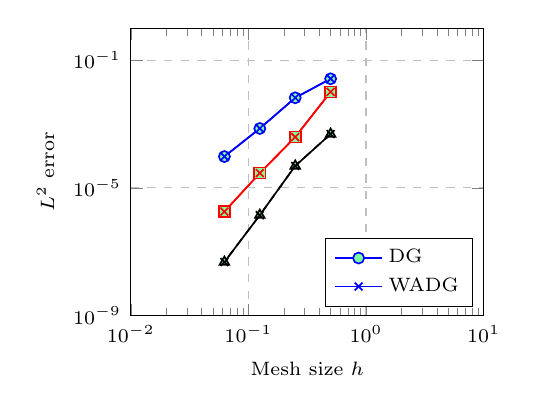
\begin{tikzpicture}
\begin{loglogaxis}[
	legend cell align=left,
	width=.5\textwidth,
%    title={Convergence},
    xlabel={Mesh size $h$},
    ylabel={$L^2$ error},
    xmin=.01, xmax=10,
    ymin=1e-9, ymax=1,        
    legend pos=south east,
    xmajorgrids=true,
    ymajorgrids=true,
    grid style=dashed,
] 
\addplot+[color=blue,mark=*,mark options={fill=markercolor},semithick]
coordinates{(0.5,0.026045)(0.25,0.00661508)(0.125,0.000722446)(0.0625,9.5217e-05)};
\addplot+[color=blue,mark=x,mark options={solid,fill=markercolor},semithick]
coordinates{(0.5,0.0260431)(0.25,0.00661506)(0.125,0.000722445)(0.0625,9.5217e-05)};

\addplot+[color=red,mark=square*,mark options={fill=markercolor},semithick]
coordinates{(0.5,0.0101239)(0.25,0.000387682)(0.125,2.88879e-05)(0.0625,1.78875e-06)};
\addplot+[color=red,mark=x,mark options={solid,fill=markercolor},semithick]
coordinates{(0.5,0.0101238)(0.25,0.000387682)(0.125,2.88879e-05)(0.0625,1.78875e-06)};

\addplot+[color=black,mark=triangle*,mark options={fill=markercolor},semithick]
coordinates{(0.5,0.000483144)(0.25,4.84164e-05)(0.125,1.38952e-06)(0.0625,4.71587e-08)};
\addplot+[color=black,mark=x,mark options={solid,fill=markercolor},semithick]
coordinates{(0.5,0.000483096)(0.25,4.84162e-05)(0.125,1.38952e-06)(0.0625,4.71587e-08)};
\legend{DG,WADG}
\end{loglogaxis}
\end{tikzpicture}
}
\caption{Optimal $L^2$ convergence rates observed for curvilinear meshes.  }
\end{figure}
}

%\frame{
%\frametitle{Curvilinear meshes: DG eigenvalues (circular domain)}
%\vspace{-1.5em}
%\begin{figure}
%\centering
%\subfloat[Central fluxes]{
%\includegraphics[width=.33\textwidth]{figs/eigstau0.png}
%}
%\subfloat[${\rm Im}\LRp{\lambda_i}$ for central fluxes]{
%\includegraphics[width=.33\textwidth]{figs/eigstau0imag.png}
%}
%\subfloat[Upwind fluxes]{
%\includegraphics[width=.33\textwidth]{figs/eigstau1.png}
%}
%%\caption{Spectra of discretized wave equation using DG and WADG for $N=3$.  Both central ($\tau = 0$) and dissipative ($\tau = 1$) numerical fluxes are shown.}
%\end{figure}
%\begin{itemize}
%\item Energy stability requires quadrature, skew-symmetric formulation
%\begin{align*}
%\int_{D^k}\pd{p}{t}{} q &= \int_{D^k} -\bm{u}\cdot \Grad q  + \frac{1}{2}\int_{\partial D^k} \LRp{2\avg{\bm{u}}\cdot{\bm{n}} + \tau_p\jump{p}} q\\
%\int_{D^k}\pd{\bm{u}}{t}{} \bm{v} &= \int_{D^k} \Grad p \cdot \bm{v} + \frac{1}{2}\int_{\partial D^k} \LRp{\jump{p} + \tau_u\jump{\bm{u}}\cdot\bm{n}} \bm{v}
%\end{align*}
%\end{itemize}
%}


%\frame{
%\frametitle{Three-dimensional curvilinear meshes}
%\setcounter{subfigure}{0}
%\begin{figure}
%\centering
%\subfloat[Planar initial mesh]{
%\includegraphics[width=.325\textwidth]{figs/spherePlanar1.png}
%}
%\hspace{.25em}
%\subfloat[Curved initial mesh]{
%\includegraphics[width=.3\textwidth]{figs/sphereCurved1.png}
%}
%\hspace{.25em}
%\subfloat[Curved refined mesh]{
%\includegraphics[width=.3\textwidth]{figs/sphereCurved2.png}
%}
%\caption{Meshes constructed using Gordon-Hall blending.}
%\end{figure}
%}
%
%\frame{
%\frametitle{Convergence on three-dimensional curvilinear meshes}
%
%\begin{figure}
%\centering
%%\vspace{-1em}
%\subfloat{
%\raisebox{2em}{
%\includegraphics[width=.35\textwidth]{figs/sphereCurved2.png}
%}
%}
%\hspace{.5em}
%\subfloat{
%\begin{tikzpicture}
%\begin{loglogaxis}[
%	legend cell align=left,
%	legend style={font=\tiny},
%	width=.575\textwidth,
%%    xlabel={Degrees of freedom},
%    xlabel={Mesh size $h$},
%    ylabel={$L^2$ error},
%%    xmin=400, xmax=2e6,
%    xmin=5e-2, xmax=1.25,
%    ymin=1e-9, ymax=.1,        
%    legend pos=south east,
%    xmajorgrids=true,
%    ymajorgrids=true,
%    grid style=dashed,
%    cycle list name=color list]
%] 
%\addplot+[color=blue,mark=*,mark options={fill=markercolor},semithick]
%coordinates{(1,0.0138761)(0.499567,0.00549824)(0.1682,9.03376e-05)(0.0830612,7.85662e-06)};
%
%\addplot+[color=red,mark=square*,mark options={fill=markercolor},semithick]
%coordinates{(1,0.00407636)(0.499567,0.000325115)(0.1682,3.81903e-06)(0.0830612,2.07829e-07)};
%
%\addplot+[color=black,mark=triangle*,mark options={fill=markercolor},semithick]
%coordinates{(1,0.000836237)(0.499567,4.83058e-05)(0.1682,1.00745e-07)};
%
%\addplot+[color=magenta,mark=diamond*,mark options={fill=markercolor},semithick]
%coordinates{(1,0.000232785)(0.499567,3.13379e-06)(0.1682,7.82233e-09)};
%
%\logLogSlopeTriangleFlip{0.3}{0.15}{0.52}{3}{blue};
%\logLogSlopeTriangleFlip{0.3}{0.15}{0.32}{4}{red};
%\logLogSlopeTriangleFlip{0.475}{0.125}{0.26}{5}{black};
%\logLogSlopeTriangle{0.55}{0.15}{0.1}{5.5}{magenta};
%
%%\logLogSlopeTriangleNeg{0.85}{0.15}{0.55}{-1}{blue};
%%\logLogSlopeTriangleNeg{0.85}{0.15}{0.39}{-4/3}{red};
%%\logLogSlopeTriangleFlipNeg{0.75}{0.15}{0.25}{-5/3}{black};
%%\addplot+[color=cyan,mark=diamond*,mark options={fill=markercolor},semithick]
%%coordinates{(2688,0.00017551)(21560,1.97403e-06)(564872,9.37127e-09)};
%%\legend{N=2,N=3, N=4,N=5}
%\end{loglogaxis}
%\end{tikzpicture}
%
%}
%\end{figure}
%\vspace{-.5em}
%\begin{itemize}
%\item Radially symmetric pressure solution $p(\bm{x},t) = \frac{\sin(\pi r)}{\pi r} \cos(\pi t)$.
%\vspace{.5em}
%\item Theoretical $O(h^{N+1/2})$ convergence of $L^2$ error observed. 
%\end{itemize}
%}

\frame{
\frametitle{Acoustics: curved meshes + heterogeneous media}
\setcounter{subfigure}{0}
\vspace{-1em}
\begin{figure}
\centering
\hspace{-2em}
\only<1->{\subfloat[Wavespeed $c^2(\bm{x})$]{\includegraphics[width=.375\textwidth]{figs/c2sphere.png}}}
\hspace{-4em}
\begin{overlayarea}{.6\textwidth}{.55\textheight}
\subfloat[Pressure isovalues at $t = .6$]{\includegraphics[width=.75\textwidth]{figs/p6.png}}
\end{overlayarea}
\end{figure}
\vspace{1em}
\begin{center}
Straightforward to combine curved elements and heterogeneous media\\with no additional cost.
\end{center}
}

\section{Elastic wave propagation}

\begin{frame}[noframenumbering]
    \frametitle{Outline}
    \tableofcontents[currentsection]
\end{frame}

\frame{
\frametitle{Matrix-valued weights and elastic wave propagation}
\begin{itemize}
\item Symmetric velocity-stress form of linear elasticity ($\bm{A}_i$ constant)
\begin{align*}
\rho\pd{\bm{v}}{t}{} = \sum_{i=1}^d \bm{A}_i^T \pd{\bm{\sigma}}{\bm{x}_i}{}, \qquad \bm{C}^{-1}\pd{\bm{\sigma}}{t}{} = \sum_{i=1}^d \bm{A}_i \pd{\bm{v}}{\bm{x}_i}{}.
\end{align*}
\item DG formulation based on penalty fluxes, matrix-weighted mass matrix
\[
{\bm{M}_{\bm{C}^{-1}}} = \LRp{\begin{array}{ccc}
\bm{M}_{C^{-1}_{11}} & \ldots & \bm{M}_{C^{-1}_{1d}}\\
\vdots & \ddots & \vdots\\
\bm{M}_{C^{-1}_{d1}} & \ldots & \bm{M}_{C^{-1}_{dd}}\\
\end{array}}
\]
%\begin{align*}
%\LRp{\rho\pd{\bm{v}}{t}{},\bm{w}} &= \LRp{\sum_{i=1}^d \bm{A}_i^T \pd{\bm{\sigma}}{\bm{x}_i}{},\bm{w} }+ \frac{1}{2}\LRa{\LRp{\bm{A}_n^T\jump{\bm{\sigma}} + \tau_v\bm{A}_n^T\bm{A}_n\jump{\bm{v}}},\bm{w}} \\
%\LRp{\bm{C}^{-1}\pd{\bm{\sigma}}{t}{}, \bm{q}}&= \LRp{\sum_{i=1}^d \bm{A}_i \pd{\bm{v}}{\bm{x}_i}{},\bm{q}} + \frac{1}{2}\LRa{\LRp{\bm{A}_n\jump{\bm{v}} + \tau_\sigma\bm{A}_n\bm{A}_n^T\jump{\bm{\sigma}}},\bm{q}} \\.
%\end{align*}
\item Weight-adjusted approximation for $\bm{C}^{-1}$ decouples each component
\[
\bm{M}_{\bm{C}^{-1}}^{-1} \approx \LRp{\bm{I}\otimes \bm{M}^{-1}} \bm{M}_{\bm{C}} \LRp{\bm{I} \otimes\bm{M}^{-1}}.
\]
%\item Reduces to Kronecker product $\bm{M}_{\bm{C}^{-1}}^{-1} = \bm{C}^{-1}\otimes \bm{M}^{-1}$ for constant $\bm{C}^{-1}$.
\end{itemize}
}

\frame{
\frametitle{Elastic wave propagation: convergence}
\setcounter{subfigure}{0}
\begin{itemize}
\item Convergence for harmonic oscillation, Rayleigh, Lamb, and Stoneley waves: between $O(h^{N+1})$ and $O(h^{N+1/2})$.  
\vspace{1em}
\item $\bm{\sigma}$ error grows as $\nor{\bm{C}^{-1}}\rightarrow \infty$ (e.g.\ incompressible limit $\lambda/\mu \rightarrow \infty$).  
\end{itemize}
\vspace{-1em}
\begin{figure}
\centering
\subfloat[Stoneley wave]{
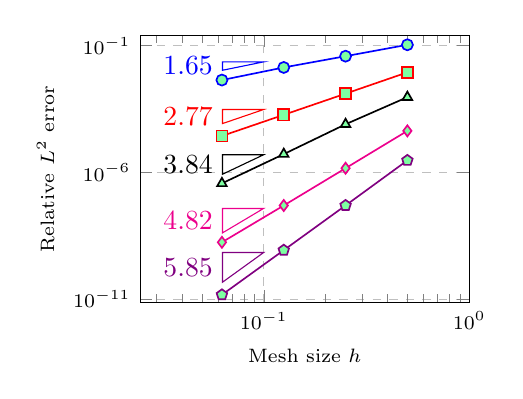
\begin{tikzpicture}
\begin{loglogaxis}[
    legend cell align=left,
    legend style={legend pos=south east, font=\tiny},
    width=.475\textwidth,
    xlabel={Mesh size $h$},
    ylabel={Relative $L^2$ error}, 
    xmin=.025, xmax=1,
    ymin=.75e-11, ymax=.25,
    xmajorgrids=true,
    ymajorgrids=true,
    grid style=dashed,
] 

\addplot[color=blue,mark=*,semithick, mark options={fill=markercolor}]
coordinates{(0.5,0.108456)(0.25,0.0385149)(0.125,0.0138288)(0.0625,0.0043988)};    
\logLogSlopeTriangleFlip{0.375}{0.125}{0.87}{1.65}{blue}

\addplot[color=red,mark=square*,semithick, mark options={fill=markercolor}]
coordinates{(0.5,0.00887301)(0.25,0.00128102)(0.125,0.000186756)(0.0625,2.73376e-05)};    
\logLogSlopeTriangleFlip{0.375}{0.125}{0.67}{2.77}{red}

\addplot[color=black,mark=triangle*,semithick, mark options={fill=markercolor}]
coordinates{(0.5,0.000930299)(0.25,7.92165e-05)(0.125,5.2534e-06)(0.0625,3.67676e-07)};    
\logLogSlopeTriangleFlip{0.375}{0.125}{0.48}{3.84}{black}

\addplot[color=magenta,mark=diamond*,semithick, mark options={fill=markercolor}]
coordinates{(0.5,4.34823e-05)(0.25,1.45784e-06)(0.125,4.92754e-08)(0.0625,1.74105e-09)};   
\logLogSlopeTriangleFlip{0.375}{0.125}{0.26}{4.82}{magenta}

\addplot[color=violet,mark=pentagon*,semithick, mark options={fill=markercolor}]
coordinates{(0.5,2.97005e-06)(0.25,4.94512e-08)(0.125,8.48451e-10)(0.0625,1.47109e-11)};  
\logLogSlopeTriangleFlip{0.375}{0.125}{0.075}{ 5.85}{violet}

%\node at (axis cs:.03,6.8e-10) {$u$ discontinuous};
%\legend{$N=1$,$N=2$,$N=3$,$N=4$,$N=5$}
\end{loglogaxis}
\end{tikzpicture}
}
\subfloat[$\nor{\bm{C^{-1}}}\rightarrow \infty$, $N=3, h = 1/8$.]{
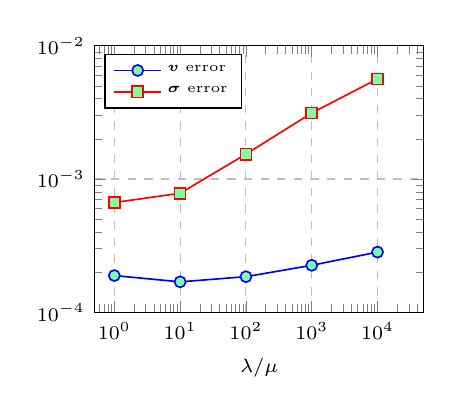
\begin{tikzpicture}
\begin{loglogaxis}[
    legend cell align=left,
    legend style={legend pos=north west, font=\tiny},
    width=.475\textwidth,
    xlabel={$\lambda / \mu$},
%    ylabel={Relative $L^2$ error}, 
    xmin=.5, xmax=5e4,
    ymin=1e-4, ymax=1e-2,
    xmajorgrids=true,
    ymajorgrids=true,
    grid style=dashed,
] 

\addplot[color=blue,mark=*,semithick, mark options={fill=markercolor}]
coordinates{(1,0.00018867)(10,0.00016925)(100,0.00018509)(1000,0.0002252)(10000,0.00028301)};

\addplot[color=red,mark=square*,semithick, mark options={fill=markercolor}]
coordinates{(1,0.00066596)(10,0.00078157)(100,0.0015353)(1000,0.0031239)(10000,0.0056341)};

\legend{$\bm{v}$ error, $\bm{\sigma}$ error }
\end{loglogaxis}
\end{tikzpicture}
}
\end{figure}
%\item Single precision energy stability 
}
%
%\frame{
%\frametitle{Elastic wave propagation: stiff inclusion}
%\begin{figure}
%\centering
%\includegraphics[width=.55\textwidth]{figs/inclusion_aligned.png}\\
%\includegraphics[width=.55\textwidth]{figs/inclusion_aligned_shear.png}
%\caption{Blah}
%\end{figure}
%}

\frame{
\frametitle{Elastic wave propagation: anisotropy}
\setcounter{subfigure}{0}
\vspace{.5em}
Simple implementation for anisotropy - fluxes independent of $\bm{C}$. 
\vspace{-.5em}
\begin{figure}
\centering
\subfloat[Vertical velocity, $t=30\mu s$]{\includegraphics[height=.525\textheight]{figs/aniso1.png}}
\subfloat[Vertical velocity, $t=60 \mu s$]{\includegraphics[height=.526\textheight]{figs/aniso2.png}}
\caption{Heterogeneous media: transverse isotropy ($x < 0$) and isotropy ($x > 0$).}
\end{figure}

\let\thefootnote\relax\footnotetext{\tiny Komatitsch, Barnes, Tromp 2000. Simulation of anisotropic wave propagation based upon a spectral element method.}
}

\frame{
\frametitle{Elastic wave propagation: acoustic-elastic coupling}
\setcounter{subfigure}{0}

\begin{itemize}
\item Interface jumps become residuals of continuity conditions:
\[
\bm{\sigma} \cdot \bm{n} = p\bm{n}, \qquad \bm{v}\cdot{\bm{n}} = \bm{u}\cdot\bm{n}.
\]
\item Energy stable for arbitrary heterogeneous media.  
\end{itemize}
\vspace{-.5em}
\begin{overlayarea}{\textwidth}{.65\textheight}
\begin{figure}
\centering
%\only<1>{\subfloat[Low order $c^2(\bm{x}), \mu(\bm{x})$]{\includegraphics[width=.3825\textwidth]{figs/c2muP0ref.png}}
%\hspace{1.5em}
%\subfloat[${\rm tr}(\bm{\sigma})$]{\includegraphics[width=.4\textwidth]{figs/acousticElasticPulseP0ref.png}}
%\caption{Acoustic-elastic waves from a Ricker pulse ($N=5$, $h = 1/32$).}
%}

\only<1>{\subfloat[Low order $c^2(\bm{x}), \mu(\bm{x})$]{\includegraphics[width=.3825\textwidth]{figs/c2muP0.png}}
\hspace{1.5em}
\subfloat[${\rm tr}(\bm{\sigma})$]{\includegraphics[width=.4\textwidth]{figs/acousticElasticPulseP0.png}}
\caption{Acoustic-elastic waves from a Ricker pulse ($N=10$, $h = 1/16$).}
}

\only<2>{\subfloat[High order $c^2(\bm{x}), \mu(\bm{x})$]{\includegraphics[width=.3825\textwidth]{figs/c2mu.png}}
\hspace{1.5em}
\subfloat[${\rm tr}(\bm{\sigma})$]{\includegraphics[width=.4\textwidth]{figs/acousticElasticPulseP10.png}}
\caption{Acoustic-elastic waves from a Ricker pulse ($N=10$, $h = 1/16$).}
}

\end{figure}
\end{overlayarea}

\let\thefootnote\relax\footnotetext{\tiny Ye et al.\ 2016. A DG method with a modified penalty flux for the propagation and scattering of acousto-elastic waves.}
}

\frame{
\frametitle{Elastic wave propagation: 3D isotropic media}
\setcounter{subfigure}{0}
\begin{figure}
\begin{overlayarea}{\textwidth}{.75\textheight}
\centering
\only<1>{
\subfloat[Computational mesh]{\includegraphics[width=.475\textwidth]{figs/cubeSplitFine.png}}
\subfloat[Piecewise constant $\bm{C}(\bm{x})$]{\includegraphics[width=.475\textwidth]{figs/pplanec0.png}}
}
\only<2>{
\subfloat[High order $\bm{C}(\bm{x})$]{\includegraphics[width=.475\textwidth]{figs/pplanew0.png}}
\subfloat[Piecewise constant $\bm{C}(\bm{x})$]{\includegraphics[width=.475\textwidth]{figs/pplanec0.png}}
}
\end{overlayarea}
\caption{${\rm tr}(\bm{\sigma})$ with $\mu(\bm{x}) = 1+ H(y) + \frac{1}{2}\cos(3\pi x)\cos(3\pi y)\cos(3\pi z)$, $N=5$.}
\end{figure}
}

\frame{
\frametitle{Summary and acknowledgements}

\begin{itemize}
\item Weight-adjusted DG (WADG) for acoustic and elastic wave propagation in heterogeneous media and curved meshes.
\vspace{.5em}
\item Energy stability and high order accuracy with low storage.
\vspace{.5em}
\item Future work: 
\vspace{.5em}
\begin{itemize}
%\item Anisotropic wave equations
%\vspace{.25em}
\item Reduced complexity algorithms using the Bernstein-Bezier basis.
\vspace{.25em}
\item Reducing high order stiffness.
\end{itemize}
\end{itemize}
\vspace{.5em}
\begin{center}
Thanks to TOTAL E\&P Research and Technology USA\\ for their support of this work!
\end{center}

\let\thefootnote\relax\footnotetext{\tiny Chan, et al.\ 2016.  {Weight-adjusted DG methods: wave propagation in heterogeneous media} (arXiv).}
\let\thefootnote\relax\footnotetext{\tiny Chan, et al.\ 2016.  {Weight-adjusted DG methods: curvilinear meshes} (arXiv).  }
\let\thefootnote\relax\footnotetext{\tiny Chan 2017.  Weight-adjusted DG methods: matrix-valued weights and elastic wave prop.\ in heterogeneous media (arXiv).}
\let\thefootnote\relax\footnotetext{\tiny Chan, Warburton 2015.  {GPU-accelerated Bernstein-Bezier discontinuous Galerkin methods for wave propagation} (SISC).}
}

%\frame{
%\begin{center}
%The authors thank TOTAL E\&P Research and Technology USA\\
%for their generous support of this work.
%\end{center}
%\let\thefootnote\relax\footnotetext{\tiny Chan, Warburton 2015. {GPU-accelerated Bernstein-Bezier DG methods for wave problems}.}
%\let\thefootnote\relax\footnotetext{\tiny Chan, Warburton 2015.  A short note on a Bernstein-Bezier basis for the pyramid.  (SISC, accepted)}
%\let\thefootnote\relax\footnotetext{\tiny Chan, et al.\ 2016.  {WADG methods I: wave propagation in heterogeneous media}.  In preparation.}
%\let\thefootnote\relax\footnotetext{\tiny Chan, et al.\ 2016.  {WADG methods II: curvilinear meshes}.  In preparation.}
%}
%% =================== extra slides =======================

\begin{frame}[noframenumbering]
\frametitle{Additional slides }

\end{frame}

%\frame[noframenumbering]{
%\frametitle{Effect of conservation on shock speeds}
%
%\begin{itemize}
%\item Weighted Burgers' equation, $w(x)$ curves characteristic lines.
%\[
%w(x)\pd{u}{t}{} + \frac{1}{2}\pd{u^2}{x}{} = 0.
%\]
%\item WADG yields high order convergence, correct shock speed for both $w(x)$ smooth, discontinuous (within an element).
%\end{itemize}
%%\vspace{-1em}
%\begin{overlayarea}{\textwidth}{.55\textheight}
%\only<1>{
%\begin{figure}
%\centering
%\subfloat[Smooth solution]{\includegraphics[width=.4\textwidth]{figs/burgersSmooth2.png}}
%\hspace{1em}
%\subfloat[Shock solution]{\includegraphics[width=.39\textwidth]{figs/burgersShock2.png}}
%\end{figure}
%}
%\only<2>{
%\vspace{2em}
%\begin{center}
%Best guess: {where} and {what} is locally conserved matters;\\ non-conservation of \textit{nonlinear flux} results in incorrect shock speeds.  
%\end{center}
%}
%\end{overlayarea}
%}


\frame[noframenumbering]{
\frametitle{Bernstein-Bezier DG methods}

\begin{itemize}
\item $O(N^6)$ cost in 3D ($O(N^4)$ with tensor product) vs $O(N^3)$ dofs.
\item Sparse Bernstein-Bezier operators ($(d+1)$ non-zeros per row).
\item Optimal $O(N^3)$ application of derivative and lift.  
\end{itemize}

\begin{figure}
\begin{overlayarea}{.875\textwidth}{.5\textheight}
\only<1>{
\centering
\subfloat{\includegraphics[width=.275\textwidth]{figs/bern1D.pdf}}
\subfloat{\includegraphics[width=.375\textwidth]{figs/bern2D.png}}
\subfloat{\includegraphics[width=.375\textwidth]{figs/bern3D.png}}
\caption{Bernstein bases in one, two, and three dimensions.}
}
\only<2>{
\centering
\subfloat[Derivative operator]{\includegraphics[height=.425\textheight]{figs/spyD_BB.eps}}
\hspace{3em}
\subfloat[$\bm{E}_{N-1}^N$]{\includegraphics[height=.425\textheight]{figs/spyE1.eps}}
\caption{Sparse Bernstein derivative and degree elevation matrices. }
}
\only<3>{
\centering
\subfloat{\includegraphics[width=.33\textwidth]{figs/bern_lift_1.pdf}}
\subfloat{\includegraphics[width=.33\textwidth]{figs/bern_lift_2.pdf}}
\subfloat{\includegraphics[width=.33\textwidth]{figs/bern_lift_3.pdf}}
\caption{Optimal-complexity ``slice-by-slice'' application of Bernstein lift.}
}
\only<4>{
\centering
\begin{tikzpicture}
\begin{axis}[
	width=.525\textwidth,
	legend cell align=left,
	%title={BB speedup over Naive nodal},
	title={BB speedup (optimal lift) over nodal},
	xlabel={Degree $N$},
	ylabel={Speedup},
	xmin=.5, xmax=9.5,
	ymin=0,ymax=8,%17.5,	
        ybar=2*\pgflinewidth,
    bar width=3pt,
	xtick={1,2,3,4,5,6,7,8,9},
	ymin=0,
	legend pos=north west,
	legend style={font=\tiny},
	ymajorgrids=true,
	grid style=dashed,
] 
%speedup V/S
\addplot table[x=N, y=V] from \runtimeOptNaive;
\addplot table[x=N, y=S] from \runtimeOptNaive;
\addplot table[x=N, y=T] from \runtimeOptNaive;
%\addplot table[x=N, y=Vopt] from \datatable;
\addplot+[draw=black,line legend, very thick,smooth,dashed] coordinates{(0,1)(10,1)};

%\legend{Volume, Surface, Total, Reference (no speedup)}
\legend{Volume, Surface, Total}
\end{axis}
\end{tikzpicture}
}
\end{overlayarea}
\end{figure}
}


\bibliographystyle{plain}
{\scriptsize
\bibliography{pyramids}
}

\end{document}
